\documentclass[border=16pt,tikz]{standalone}
\usepackage{tikz}
\usetikzlibrary{arrows.meta,bending}
\usepackage[margin=2cm]{geometry}
\pagestyle{empty} % Remove page numbers
\begin{document}

% Define player names
\def\PlayerA{A}
\def\PlayerB{B}
\def\PlayerC{C}
\def\PlayerD{D}

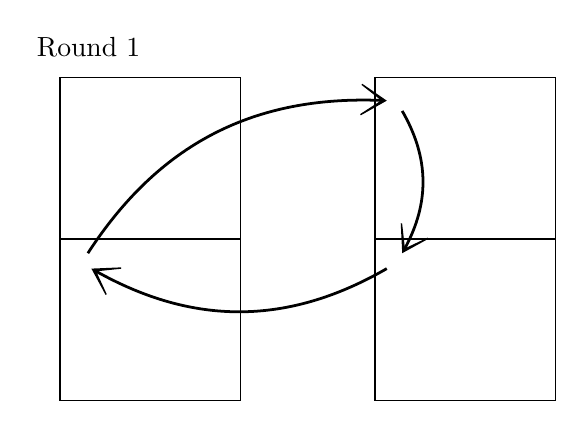
\begin{tikzpicture}
  % Define a custom arrow tip
  \tikzset{custom arrow/.style={
    -{Stealth[length=16pt,width=20pt, inset=14pt]}
  }}
  
% Round 1
\node[anchor=east] at (1.14375,4.5) {Round 1};
% First table tennis table 
\draw (0,0) rectangle (2.2875,4.11);
\draw (0,2.055) -- (2.2875,2.055); % Horizontal net line
\node[anchor=north west] at (0.15,1.875) (D1) {\PlayerD}; 
\node[anchor=north west] at (0.15,3.93) (A1) {\PlayerA}; 

% Second table tennis table 
\draw (4,0) rectangle (6.2875,4.11);
\draw (4,2.055) -- (6.2875,2.055); % Horizontal net line
\node[anchor=north west] at (4.15,1.875) (C1) {\PlayerC}; 
\node[anchor=north west] at (4.15,3.93) (B1) {\PlayerB}; 

% Add curved arrows
\draw[custom arrow, bend left, line width=1.0pt] (B1) to (C1);
\draw[custom arrow, bend left, line width=1.0pt] (C1) to (D1);
\draw[custom arrow, bend left, line width=1.0pt] (D1) to (B1);

\end{tikzpicture}
\end{document}
